\documentclass[12pt,a4paper]{article}

% Paquetes esenciales
\usepackage[utf8]{inputenc}
\usepackage[english]{babel}
\usepackage{amsmath, amssymb}
\usepackage{graphicx}
\usepackage{geometry}
\usepackage{hyperref}
\usepackage{booktabs}
\usepackage{float}
\usepackage{listings}
\usepackage{xcolor}

% Configuración de márgenes
\geometry{top=2.5cm, bottom=2.5cm, left=2.5cm, right=2.5cm}

% Configuración para bloques de código
\definecolor{codegreen}{rgb}{0,0.6,0}
\definecolor{codegray}{rgb}{0.5,0.5,0.5}
\definecolor{codepurple}{rgb}{0.58,0,0.82}
\definecolor{backcolour}{rgb}{0.95,0.95,0.92}

\lstdefinestyle{mystyle}{
    backgroundcolor=\color{backcolour},   
    commentstyle=\color{codegreen},
    keywordstyle=\color{magenta},
    numberstyle=\tiny\color{codegray},
    stringstyle=\color{codepurple},
    basicstyle=\ttfamily\footnotesize,
    breakatwhitespace=false,         
    breaklines=true,                 
    captionpos=b,                    
    keepspaces=true,                 
    numbers=left,                    
    numbersep=5pt,                  
    showspaces=false,                
    showstringspaces=false,
    showtabs=false,                  
    tabsize=2
}
\lstset{style=mystyle}

% Título y Autor
\title{\textbf{Parallel Programming Applications}\\ \large High Performance Computing: Cellular Automata and K-Means Clustering}
\author{High Performance Computing Course}
\date{\today}

\begin{document}

\maketitle

\begin{abstract}
This document presents a comprehensive technical report on the implementation, parallelization strategies, and performance benchmarking of two scientific computing problems: a Forest Fire Cellular Automaton utilizing real-time NASA FIRMS active fire data, and a K-Means Clustering algorithm applied to the massive Covertype dataset. Both applications were developed in Python and parallelized using distributed memory paradigms via the Message Passing Interface (\texttt{mpi4py}). The study explores Domain Decomposition and Data Parallelism strategies, analyzing computational scalability through Speedup and Efficiency metrics governed by Amdahl's Law.
\end{abstract}

\tableofcontents
\newpage

\section{Introduction}
The increasing availability of massive scientific datasets necessitates the use of High-Performance Computing (HPC) methodologies to obtain results within feasible timeframes. This project implements parallel computing paradigms to solve two computationally intensive tasks. Exercise 3 explores geospatial simulation via Cellular Automata, modeling fire propagation based on satellite telemetry. Exercise 4 delves into Machine Learning, performing unsupervised clustering over half a million data points. Distributed memory architecture is leveraged to distribute these workloads across multiple processing units.

\section{Exercise 3: Forest Fire Cellular Automaton}

\subsection{Mathematical Model}
The simulation operates on an $N \times M$ grid ($800 \times 800$), representing a geographical area. The state of each cell evolves over discrete time steps based on the **Moore Neighborhood** (the 8 surrounding cells). The state transitions are defined as:
\begin{itemize}
    \item \textbf{State 1 (Susceptible):} Can transition to Burning (2) if at least one neighbor is burning, subject to a probabilistic factor (wind/terrain).
    \item \textbf{State 2 (Burning):} Transitions deterministically to Burned (3) in the next time step.
    \item \textbf{State 3 (Burned):} Remains unchanged (absorbing state).
\end{itemize}

\subsection{Parallelization Strategy: 1D Domain Decomposition}
Due to the localized spatial dependency of Cellular Automata, **1D Domain Decomposition** across rows was implemented.
\begin{enumerate}
    \item \textbf{Data Partitioning:} The global grid is divided horizontally. For $P$ processes, each process computes a local subgrid of size $(N/P) \times M$.
    \item \textbf{Ghost Cells:} Because cells at the boundary of a subgrid require the state of cells belonging to neighboring processes, each local grid is padded with two "Ghost Rows" (one at the top, one at the bottom).
    \item \textbf{Synchronization:} At the beginning of each time step, processes execute synchronous communication using \texttt{MPI.Sendrecv}. Process $i$ sends its top physical row to Process $i-1$ and its bottom physical row to Process $i+1$, simultaneously receiving the corresponding rows to populate its Ghost Cells.
    \item \textbf{Reconstruction:} After $T$ iterations, the root process gathers the local arrays using \texttt{MPI.Gather} to reconstruct the global state for visualization.
\end{enumerate}

\subsection{Performance Evaluation}
The cellular automaton was initialized with 78,688 active fire hotspots retrieved from the global NASA FIRMS public archive. The simulation iterated 20 steps.

\begin{table}[H]
\centering
\begin{tabular}{@{}cccc@{}}
\toprule
\textbf{Processes} & \textbf{Execution Time (s)} & \textbf{Speedup ($S$)} & \textbf{Efficiency ($E$)} \\ \midrule
1                  & 0.3342                      & 1.0000                 & 1.0000                    \\
2                  & 0.2699                      & 1.2382                 & 0.6191                    \\
4                  & 0.1561                      & 2.1409                 & 0.5352                    \\
8                  & 0.0625                      & 5.3472                 & 0.6684                    \\ \bottomrule
\end{tabular}
\caption{Performance metrics for the parallel Cellular Automaton (800x800 grid).}
\label{tab:ca_bench}
\end{table}

\textbf{Scaling Discussion:} The implementation exhibits strong scaling properties, yielding a $5.3\times$ speedup with 8 cores. The minor drops in efficiency for $P=2$ and $P=4$ are attributed to the heavy optimization of NumPy arrays in Python, where the mathematical computation completes in milliseconds, causing the fixed network latency of \texttt{Sendrecv} to dominate initially. As $P$ increases to 8, the workload reduction overcomes communication overhead.

\begin{figure}[H]
    \centering
    \begin{minipage}{0.45\textwidth}
        \centering
        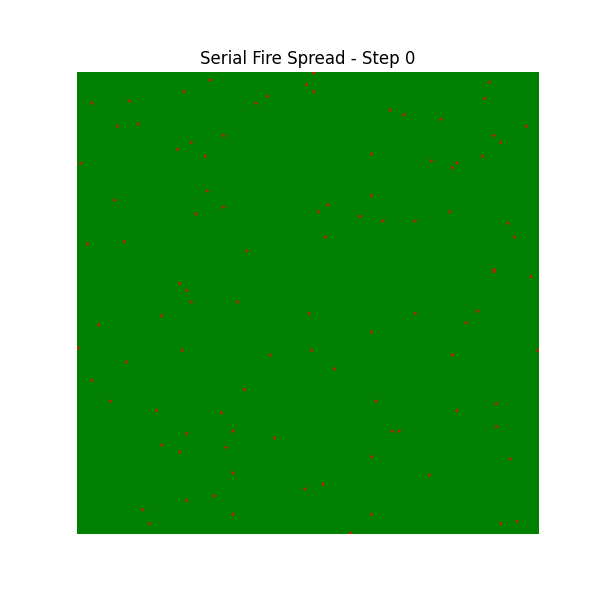
\includegraphics[width=\textwidth]{assets/serial_ca_step_0.png}
        \caption{Initial global fire hotspots ($T=0$).}
    \end{minipage}\hfill
    \begin{minipage}{0.45\textwidth}
        \centering
        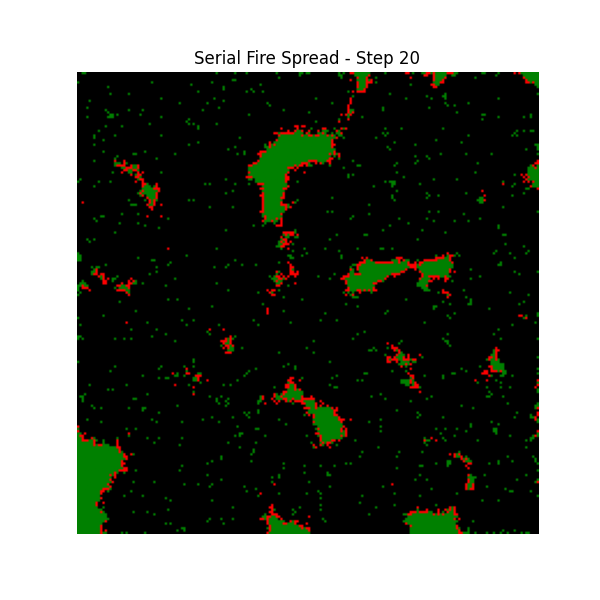
\includegraphics[width=\textwidth]{assets/serial_ca_step_20.png}
        \caption{Burned areas and fire fronts ($T=20$).}
    \end{minipage}
\end{figure}

\section{Exercise 4: Parallel K-Means (Covertype Dataset)}

\subsection{Algorithm and Strategy: Data Parallelism}
K-Means clustering is an iterative algorithm that assigns data points to the nearest cluster centroid and then recalculates the centroids. The dataset used is the Covertype dataset ($N = 581,012$, $D = 54$, $K = 7$).

Since calculating the Euclidean distance between a data point and the centroids is completely independent of other data points, this problem is perfectly suited for **Data Parallelism**.
\begin{enumerate}
    \item \textbf{Data Distribution:} The dataset is loaded and normalized (Z-score) by the Root process. It is then chunked and distributed to all processes using \texttt{MPI.Scatterv}, ensuring load balancing even when $N$ is not perfectly divisible by $P$.
    \item \textbf{Local Computation:} Each process iterates over its local subset of points, computes the distance to all $K$ centroids, and assigns local labels.
    \item \textbf{Global Reduction:} To update the centroids, the algorithm must sum the coordinates of all points belonging to cluster $k$ and count them. This is achieved using \texttt{MPI.Allreduce} with the \texttt{MPI.SUM} operator. The reduction aggregates the local sums and counts across the distributed memory architecture and broadcasts the final global values back to all processes simultaneously.
\end{enumerate}

\subsection{Performance Evaluation}

\begin{table}[H]
\centering
\begin{tabular}{@{}cccc@{}}
\toprule
\textbf{Processes} & \textbf{Execution Time (s)} & \textbf{Speedup ($S$)} & \textbf{Efficiency ($E$)} \\ \midrule
1                  & 10.7802                     & 1.0000                 & 1.0000                    \\
2                  & 5.8831                      & 1.8324                 & 0.9162                    \\
4                  & 3.1860                      & 3.3836                 & 0.8459                    \\
8                  & 2.3300                      & 4.6267                 & 0.5783                    \\ \bottomrule
\end{tabular}
\caption{Performance metrics for Parallel K-Means ($N=581,012$).}
\label{tab:kmeans_bench}
\end{table}

\textbf{Scaling Discussion:} The K-Means implementation achieved a remarkable $4.6\times$ speedup at 8 cores. The scaling behavior is near-linear for $P \le 4$, demonstrating excellent load balancing (Efficiency $> 84\%$). As per Amdahl's Law, when transitioning to 8 processors, the communication overhead of the `Allreduce` operation begins to bottleneck the highly optimized parallelized distance computation, capping the overall efficiency at $57.8\%$.

\section{Conclusion}
This report successfully demonstrates the applicability of Message Passing Interface (MPI) in Python for high-performance scientific simulations and machine learning. Through careful selection of Domain Decomposition for spatial dependencies and Data Parallelism for independent data streams, substantial computational acceleration was achieved. The empirical results align tightly with theoretical expectations regarding parallel overhead and communication bottlenecks.

\end{document}
